\section{Schritte für die Durchführung} \label{sec:steps}

Für die Umsetzung dieser Arbeit wird eine \ac{db} in PostgreSQL entwickelt, um die Information der \ac{fhir}-Profile und Konfigurationsparameter der \ac{copra}-Instanz des Staging Bereichs des \ac{dw} des \ac{diz} an der Universitätsmedizin Mainz zu speichern, und einige der Schritte des Data Mappings durchzuführen.

Die \ac{fhir}-Profile des Erweiterungsmoduls \glqq\ac{icu}\grqq{} werden analysiert, und die allgemeinen Parameter der Profile werden in der entwickelten \ac{db} gespeichert. Einige dieser Parameter werden als Hilfsmittel für die Datenzuordnung angewendet. Andere hingegen spiegeln die Attribute der Biosignaldaten in \ac{copra} wider.

Nach der Speicherung der Profile wird die Struktur der Tabellen von \ac{copra} in dem Staging Bereich des \ac{dw} analysiert. Diese beinhalten die Metadaten, wie Konfigurationsvariablen und Datentypen, und die Werte der Biosignaldaten mit den Attributen für das Data Mapping mit den \ac{fhir}-Profilen. 

Die Voraussetzungen für die Auswahl der Konfigurationsvariablen für die weitere Durchführung des Projekts werden definiert. Die ausgewählten Konfigurationsvariablen sollen patienten- oder fallbezogene sein, und mindestens 1000 validierten, aktuellen und nicht gelöschten Datensätzen in den Werttabellen beinhalten (\ref{subsec:datadef}).

Nach der Auswahl werden die entscheidenden Attribute der Konfigurationsvariablen in die vorher entwickelten PostgreSQL \ac{db} importiert. Diese Konfigurationsvariablen beinhalten die Namen von Beobachtungen und Messungen. Diese solle den \glqq Procedure\grqq{}- und \glqq Observations\grqq{}-Profilen entsprechen.

Mit den gespeicherten Informationen der \ac{fhir}-Profile und den Konfigurationsvariablen in der \ac{db} und der analysierten Datenstruktur von \ac{copra} wird das manuelle Data Mapping durchgeführt. Von diesem Prozess werden in diesem Projekt drei Schritte umgesetzt: die Datendefinition, Zuweisung der Quell- und Zielfelder, und die Programmierung der Transformationsregeln.

Der Prozess für die Verlinkung der Konfigurationsvariablen mit den \ac{fhir}-Profilen generiert einen Datensatz mit den notwendigen Attributen der Konfigurationsvariablen und der \ac{fhir}-Profile. Dieser Datensatz wird validiert, und die Maßeinheiten beider Systeme werden verglichen, um Fehler und andere Irregularitäten zu detektieren, und wenn möglich, mit der Kooperation der fachlichen Spezialisten der \ac{pdms}-Abteilung und Transformationsregeln solche Probleme zu lösen. Diese Regeln werden in dem Datensatz der zugeordneten Konfigurationsvariablen mit den \ac{fhir}-Profilen eingefügt.

Der Datensatz der zugeordneten Konfigurationsvariablen mit den \ac{fhir}-Profilen wird danach in die \ac{copra}-Instanz des Staging Bereichs des \ac{dw} angelegt, um weitere Transformationsregeln für die Erzeugung der \ac{fhir}-Ressourcen aus den Biosignaldaten von \ac{copra} zu definieren.

Mit dem Datensatz der zugeordneten Konfigurationsvariablen in dem Staging Bereich des \ac{dw} und mit der Identifikation der Felder von Quelle- und Zielsystemen werden \ac{sql}-Views in dem \ac{copra}-Instanz des Staging Bereichs programmiert, um die notwendigen Parameter der verschiedenen Tabellen zusammenzuführen. Diese Views können bei der Implementierung für die Erzeugung der \ac{fhir}-Ressourcen angewendet werden.

Ein Flussdiagramm (\ref{sec:flowdiagram}) der Ablaufschritte dieses Projekts ist in der \ref{fig:flowdiagram} dargestellt.

\clearpage

\begin{figure}[ht]
	\centering
	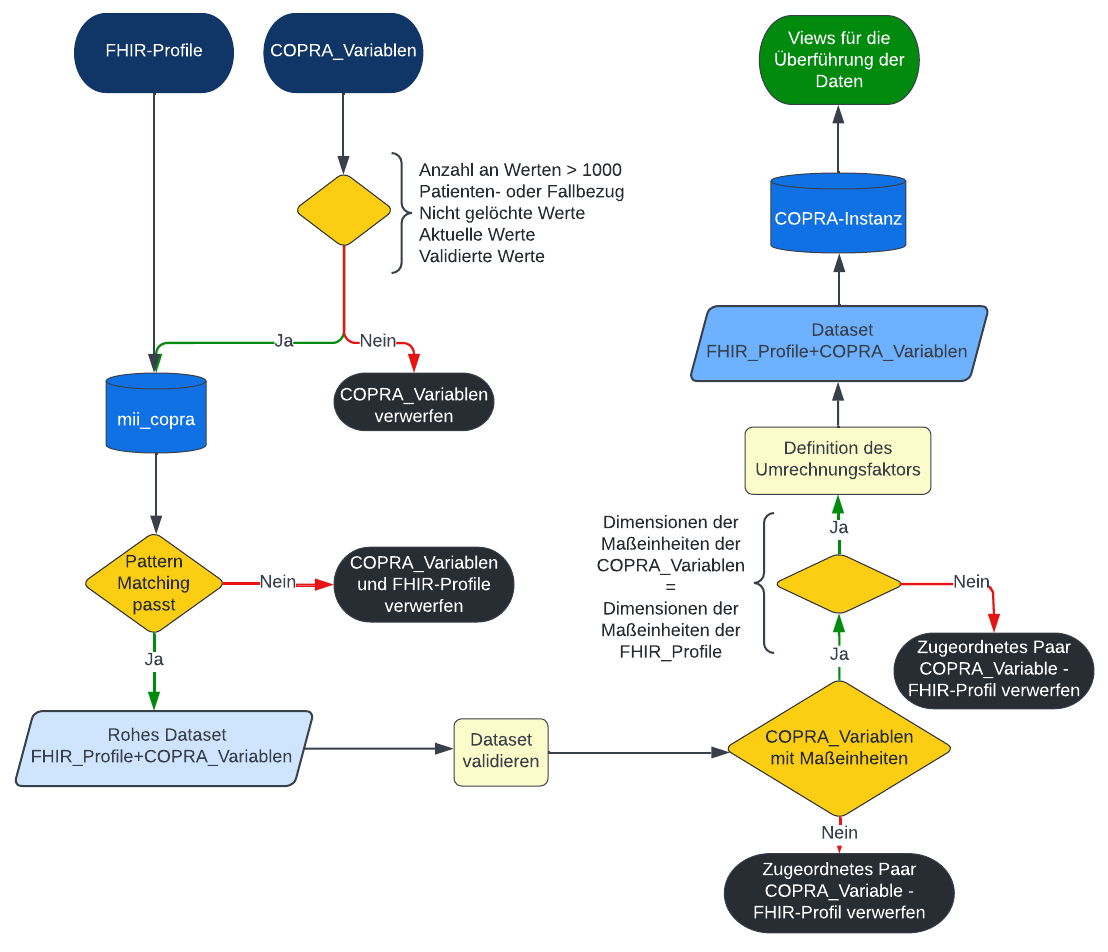
\includegraphics[height=10.5cm]{figures/thesis_flow}
	\caption[Flussdiagramm des Ablaufes des Projekts]{Flussdiagramm des Ablaufes des Projekts.}
	\label{fig:flowdiagram}
\end{figure}